Linear trap measurements have been taken twice.
The first measurement was with the subcarrier at the same offset frequency from
the carrier for each measurement.
The results generally were in line with the theory, however there were
complications with the layout that we felt should be improved on.

\section{First Experiment}

%\begin{figure}[htbp]
%    \centering
%    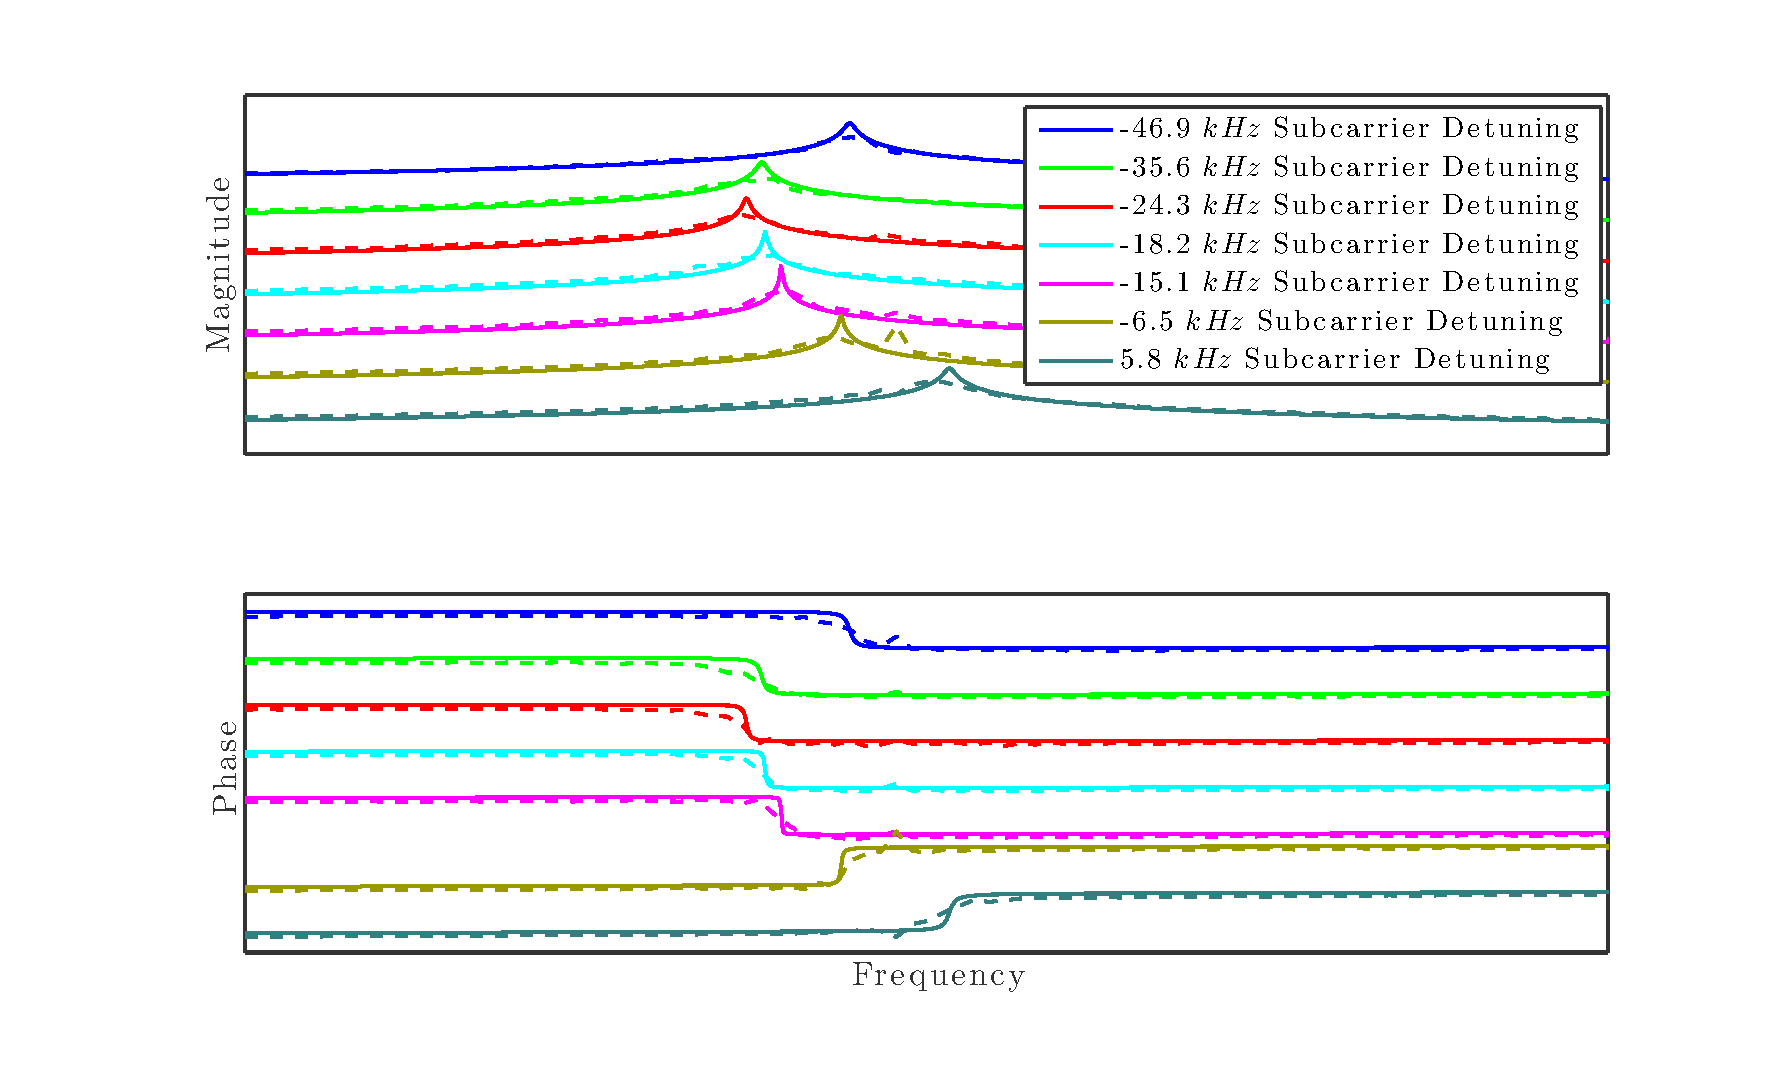
\includegraphics[width=20cm]{./figures/april_results_olgfit.eps}
%    \caption[Data Fitting of Open Loop Gain for 1st Results]{This is the open
%        loop gain fit of the last 7 measurements taken during a segment of
%        time in which the cavity was continuously locked.
%        The trap cavity had been locked for a few hours at this point and
%        seemed to have stabilized compared to earlier in the lock segment.
%        These measurements were taken no more than 5 minutes apart from each
%        other so the effects of any drifted were minimized.}
%    \label{fig:olgapril}
%\end{figure}

The first set of measurements seemed to have a large drift.
One of the reasons for this is the fact that the carrier beam was not
well aligned to the subcarrier beam causing drifts in the power ratio between
carrier and subcarrier as the overall alignment drifted.
Another complication in the first run was due to the fact that the carrier and
subcarrier beams had exactly the same polarizations which caused a strong
beat signal at $355kH\!z$. This beat signal was low enough in frequency that
it would show strongly in the resonant \ac{rfpd} output, likely causing
saturation effects in the electronics that would lead to an unpredictable
subcarrier detuning.

Despite these issues we were clearly able to observe
stable and unstable optical springs and there was a short stretch of
measurements that did line up with the model with certain assumptions
about the parameter space.


\begin{figure}[htbp]
  \label{fig:april_space1}
  \tikzsetnextfilename{april_space1}
  \begin{tikzpicture}
  \begin{axis}[
    name=plot1,
    height=8cm,
    width=14cm,
    ylabel={Resonant Frequency $(H\!z)$},
    xlabel={Subcarrier Detuning $(kH\!z)$},
    grid=major,
  ]
  \addplot[blue,very thick] table[x index=1,y index=2]
    {./matlab_traces/april_fitspace_stable.dat};
  \addplot[green,very thick] table[x index=1,y index=2]
    {./matlab_traces/april_fitspace_unstable.dat};
  \addplot[blue,only marks] table[x index=1,y index=2]
    {./matlab_traces/april_pointspace_stable.dat};
  \addplot[green,only marks] table[x index=1,y index=2]
    {./matlab_traces/april_pointspace_unstable.dat};
  \end{axis}
  \end{tikzpicture}
  \caption[Parameters from 1st Experiment]{The solid lines show the theoretical
    spring frequencies for all of the measurements that took place in a span
    of about 30 minutes during the first experiment at the end of one lock
    stretch.
    The dots correspond to the actual measurements of the optical spring at
    different subcarrier detunings. The entire space depicted is in the region
    of static stability, i.e. the optical spring provides a restoring force.
    The colors correspond to the dynamic stability of the optical spring.
    Blue is dynamically stable.
    Green is dynamically unstable.
    The carrier frequency remained at a fixed offset from the subcarrier at
    $355\, kH\!z$.
    }
\end{figure}

\begin{figure}[htbp]
  \label{fig:april_olg1}
  \tikzsetnextfilename{april_olg1}
  \begin{tikzpicture}
  \begin{semilogyaxis}[
    name=plot1,
    height=5cm,
    width=7cm,
    xmin=760,
    xmax=880,
    ylabel={Magnitude},
    grid=major,
  ]
  \addplot[blue,very thick] table[x index=0,y index=1] {./matlab_traces/april_olg_38.dat};
  \addplot[blue] table[x index=0,y index=1] {./matlab_traces/april_fit.dat};
  \addplot[red,very thick] table[x index=0,y index=1] {./matlab_traces/april_olg_39.dat};
  \addplot[red] table[x index=0,y index=3] {./matlab_traces/april_fit.dat};
  \addplot[green,very thick] table[x index=0,y index=1] {./matlab_traces/april_olg_40.dat};
  \addplot[green] table[x index=0,y index=5] {./matlab_traces/april_fit.dat};
  \end{semilogyaxis}

  \begin{semilogyaxis}[
    name=plot2,
    at=(plot1.below south), anchor=above north,
    height=5cm,
    width=7cm,
    xmin=760,
    xmax=880,
    xlabel={Frequency $(H\!z)$},
    ylabel={Magnitude},
    grid=major,
  ]
  \addplot[blue,very thick] table[x index=0,y index=1] {./matlab_traces/april_olg_41.dat};
  \addplot[blue] table[x index=0,y index=7] {./matlab_traces/april_fit.dat};
  \addplot[red,very thick] table[x index=0,y index=1] {./matlab_traces/april_olg_42.dat};
  \addplot[red] table[x index=0,y index=9] {./matlab_traces/april_fit.dat};
  \addplot[green,very thick] table[x index=0,y index=1] {./matlab_traces/april_olg_43.dat};
  \addplot[green] table[x index=0,y index=11] {./matlab_traces/april_fit.dat};
  \addplot[black,very thick] table[x index=0,y index=1] {./matlab_traces/april_olg_44.dat};
  \addplot[black] table[x index=0,y index=13] {./matlab_traces/april_fit.dat};
  \end{semilogyaxis}

  \begin{axis}[
    name=plot3,
    at=(plot1.right of east), anchor=left of west,
    height=5cm,
    width=7cm,
    xmin=760,
    xmax=880,
    ylabel={Phase},
    grid=major,
  ]
  \addplot[blue,very thick] table[x index=0,y index=2] {./matlab_traces/april_olg_38.dat};
  \addplot[blue] table[x index=0,y index=2] {./matlab_traces/april_fit.dat};
  \addplot[red,very thick] table[x index=0,y index=2] {./matlab_traces/april_olg_39.dat};
  \addplot[red] table[x index=0,y index=4] {./matlab_traces/april_fit.dat};
  \addplot[green,very thick] table[x index=0,y index=2] {./matlab_traces/april_olg_40.dat};
  \addplot[green] table[x index=0,y index=6] {./matlab_traces/april_fit.dat};
  \end{axis}
  \begin{axis}[
    name=plot4,
    at=(plot2.right of east), anchor=left of west,
    height=5cm,
    width=7cm,
    xmin=760,
    xmax=880,
    xlabel={Frequency $(H\!z)$},
    ylabel={Phase},
    grid=major,
  ]
  \addplot[blue,very thick] table[x index=0,y index=2] {./matlab_traces/april_olg_41.dat};
  \addplot[blue] table[x index=0,y index=8] {./matlab_traces/april_fit.dat};
  \addplot[red,very thick] table[x index=0,y index=2] {./matlab_traces/april_olg_42.dat};
  \addplot[red] table[x index=0,y index=10] {./matlab_traces/april_fit.dat};
  \addplot[green,very thick] table[x index=0,y index=2] {./matlab_traces/april_olg_43.dat};
  \addplot[green] table[x index=0,y index=12] {./matlab_traces/april_fit.dat};
  \addplot[black,very thick] table[x index=0,y index=2] {./matlab_traces/april_olg_44.dat};
  \addplot[black] table[x index=0,y index=14] {./matlab_traces/april_fit.dat};
  \end{axis}
  \end{tikzpicture}
    \caption[Data Fitting of Open Loop Gain for 1st Results]{This is the open
        loop gain fit of the last 7 measurements taken during a segment of
        time in which the cavity was continuously locked.
        The three traces in the top two plots are of the stable spring with
        a large negative detuning.
        They correspond to the three blue dots from figure
        \ref{fig:april_space1} with the most negative subcarrier detuning.
        The thick traces in all plots are from the measurements in the lab.
        The thin traces are of the modelled open loop gain.
        The trap cavity had been locked for a few hours at this point and
        seemed to have stabilized compared to earlier in the lock segment.
        These measurements were taken no more than 5 minutes apart from each
        other so the effects of any drifting were minimized.}
  \label{fig:aprilolg1}
\end{figure}


\section{Experimental Layout Revision}
From our first layout design there was a rather
large beat signal on the \ac{rfpd} used for generating the \ac{pdh} signal
for our locking feedback servo.
This beat signal is a result of our initial layout involving the combining of
carrier and subcarrier beams before the \ac{fi} which resulted in the two beams
having the same polarization.
This produces a beat signal of the difference in the two frequencies.
The beat signal shows up in our resonant \ac{rfpd} because we use a small
frequency offset.
We feared there could be saturations in the photodiode electronics that would
cause unpredictable electronic offsets in the trap locking feedback servo
resulting in an error on the subcarrier detuning lock point.


\section{Second Experiment}

During the second experiment we were able to observe several stable and
unstable spring as before. This time we varied the frequency offset between
carrier and subcarrier for each measurement, keeping the other settings
fixed. The data fitting proved problematic.
The stability of the optical springs were difficult to match with the theory.
We finally determined that there had to be some new physics messing with us.
We believe that the likely explanation for this is the intensity noise coupling
to optic expansion through a surface absorption on the high reflectivity
coating.
It turns out that only 5ppm absorption is required to account for the phase
discrepancy.
This is, in part, due to the high circulating power and the small
beam spot size on the cavity end mirrors.
The results of this fitting can be seen in figure \ref{fig:juneOLGresults}.

\subsection{Optic Expansion}
See section 2.8.5 of Stefan Ballmer's thesis  \cite{Ballmer:thesis} for
a thorough discussion on thermal noise couplings.
The relevant part that we are interested in is the effect of changing
the thickness of the optic itself due to thermal expansion.
We want to first consider the penetration depth $d$ of the thermal
fluctuations. This is given by,
\begin{align}
d &= \sqrt{\frac{\kappa}{2\pi fC\rho}} = 50\mu m \sqrt{\frac{400 H\!z}{f}}
\end{align}
This is nearly an order of magnitude smaller than the beam spot diameter, which
is about $320\mu m$. The change in thickness $\Delta_z$ of the optic can then
be approximated with,
\begin{align}
\Delta_z &= \left(1+\eta\right)\alpha\frac{P \delta (\mathrm{RIN}) }{2\pi ifC\rho A}
\end{align}
where $\delta$ is the absorption coefficient, $A$ is the area of the beam,
and $\eta$ is the Poisson ratio.

The majority of the change in power buildup due to cavity length is due to the
carrier beam which has a positive detuning.
Because of this detuning, expansion of the optics will shorten the cavity and
increase the intracavity power.
The intracavity power fluctuations will thus have a positive feedback and add
to the instability of the optical spring.


\begin{figure}[htbp]
  \tikzsetnextfilename{juneOLGresults}
  \begin{tikzpicture}
  \begin{loglogaxis}[
    name=plot1,
    height=7cm,
    width=14cm,
    xmin=100,
    xmax=2000,
    xtick={1e2,1e3},
    ylabel={Magnitude},
    grid=both,
  ]
  \addplot[blue,very thick,dashed] table[x index=0,y index=1]
    {./matlab_traces/juneResults13fit.dat};
  \addplot[green,very thick,dashed] table[x index=0,y index=1]
    {./matlab_traces/juneResults20fit.dat};
  \addplot[red,very thick,dashed] table[x index=0,y index=1]
    {./matlab_traces/juneResults10fit.dat};
  \addplot[teal,very thick,dashed] table[x index=0,y index=1]
    {./matlab_traces/juneResults15fit.dat};
  \addplot[magenta,very thick,dashed] table[x index=0,y index=1]
    {./matlab_traces/juneResults18fit.dat};
  \addplot[yellow,very thick,dashed] table[x index=0,y index=1]
    {./matlab_traces/juneResults19fit.dat};
  \addplot[blue,very thick] table[x index=0,y index=1] {./matlab_traces/juneResults13.dat};
  \addplot[green,very thick] table[x index=0,y index=1] {./matlab_traces/juneResults20.dat};
  \addplot[red,very thick] table[x index=0,y index=1] {./matlab_traces/juneResults10.dat};
  \addplot[teal,very thick] table[x index=0,y index=1] {./matlab_traces/juneResults15.dat};
  \addplot[magenta,very thick] table[x index=0,y index=1] {./matlab_traces/juneResults18.dat};
  \addplot[yellow,very thick] table[x index=0,y index=1] {./matlab_traces/juneResults19.dat};
  \end{loglogaxis}
  \begin{semilogxaxis}[
    name=plot2,
    at=(plot1.below south), anchor=above north,
    height=7cm,
    width=14cm,
    xmin=100,
    xmax=2000,
    xtick={1e2,1e3},
    xlabel={Frequency $(H\!z)$},
    ylabel={Phase (Deg)},
    legend style={legend pos=north west,font=\tiny},
    grid=both,
  ]
  \addplot[blue,very thick,dashed,forget plot] table[x index=0,y index=2]
    {./matlab_traces/juneResults13fit.dat};
  \addplot[green,very thick,dashed,forget plot] table[x index=0,y index=2]
    {./matlab_traces/juneResults20fit.dat};
  \addplot[red,very thick,dashed,forget plot] table[x index=0,y index=2]
    {./matlab_traces/juneResults10fit.dat};
  \addplot[teal,very thick,dashed,forget plot] table[x index=0,y index=2]
    {./matlab_traces/juneResults15fit.dat};
  \addplot[magenta,very thick,dashed,forget plot] table[x index=0,y index=2]
    {./matlab_traces/juneResults18fit.dat};
  \addplot[yellow,very thick,dashed,forget plot] table[x index=0,y index=2]
    {./matlab_traces/juneResults19fit.dat};
  \addplot[blue,very thick] table[x index=0,y index=2] {./matlab_traces/juneResults13.dat};
  \addlegendentry{DetC$=290.8kH\!z$,DetS$=-39.2kH\!z$,Pratio=3.46}
  \addplot[green,very thick] table[x index=0,y index=2] {./matlab_traces/juneResults20.dat};
  \addlegendentry{DetC$=285.0kH\!z$,DetS$=-45.0kH\!z$,Pratio=3.96}
  \addplot[red,very thick] table[x index=0,y index=2] {./matlab_traces/juneResults10.dat};
  \addlegendentry{DetC$=285.1kH\!z$,DetS$=-34.9kH\!z$,Pratio=3.50}
  \addplot[teal,very thick] table[x index=0,y index=2] {./matlab_traces/juneResults15.dat};
  \addlegendentry{DetC$=264.2kH\!z$,DetS$=-35.8kH\!z$,Pratio=3.94}
  \addplot[magenta,very thick] table[x index=0,y index=2] {./matlab_traces/juneResults18.dat};
  \addlegendentry{DetC$=238.2kH\!z$,DetS$=-21.8kH\!z$,Pratio=4.27}
  \addplot[yellow,very thick] table[x index=0,y index=2] {./matlab_traces/juneResults19.dat};
  \addlegendentry{DetC$=222.5kH\!z$,DetS$=-17.5kH\!z$,Pratio=4.42}
  \end{semilogxaxis}
  \end{tikzpicture}
    \caption[Data Fitting of Open Loop Gain for 1st Results]{This is the open
      loop gain fit for the second experiment. The solid lines are the measured
      optical spring transfer functions. The dashed lines are the corresponding
      theoretical transfer functions. In the legend, "DetC" and "DetS" stand for
      carrier and subcarrier detuning respectively. Pratio is the power ratio
      of carrier to subcarrier input power.}
  \label{fig:juneOLGresults}
\end{figure}


\begin{figure}[htbp]
  \tikzsetnextfilename{noisepassive}
  \begin{tikzpicture}
  \begin{loglogaxis}[
    height=12cm,
    width=14cm,
    xlabel={Frequency $(H\!z)$},
    ylabel={Trap Length Noise $(m/\sqrt{H\!z})$},
    xmin=10,
    xmax=6000,
    ymin=1e-16,
    ymax=1e-8,
    grid=major,
    legend cell align=left,
  ]
  \addplot[blue,very thick] table[x index=0,y index=1]
    {./matlab_traces/june_noises.dat};
  \addlegendentry{Measured Trap Length Noise}
  \addplot[red,very thick] table[x index=0,y index=5]
    {./matlab_traces/june_noises.dat};
  \addlegendentry{Trap Length Noise Without Active Feedback}
  \addplot[red,dashed,very thick] table[x index=0,y index=6]
    {./matlab_traces/june_noises.dat};
  \addlegendentry{Trap Length RMS Without Active Feedback}
  \end{loglogaxis}
  \end{tikzpicture}
  \caption[Estimate of Passively Attenuated Noise]{This is the noise budget which includes the measured
    cavity length noise with a stable optical spring.}
  \label{fig:noisepassive}
\end{figure}


